\documentclass[tikz,border=6pt]{standalone}
\usepackage{fontspec}
\setmainfont{Noto Sans}
\usepackage{amsmath}
\usepackage{tikz}
\usetikzlibrary{arrows.meta,positioning}
\definecolor{cudaG}{RGB}{118,185,0}
\definecolor{sadRed}{RGB}{200,60,50}
\definecolor{gsBlue}{RGB}{40,110,190}
\definecolor{pyYel}{RGB}{240,170,30}
\definecolor{secG}{RGB}{85,85,85}
\begin{document}
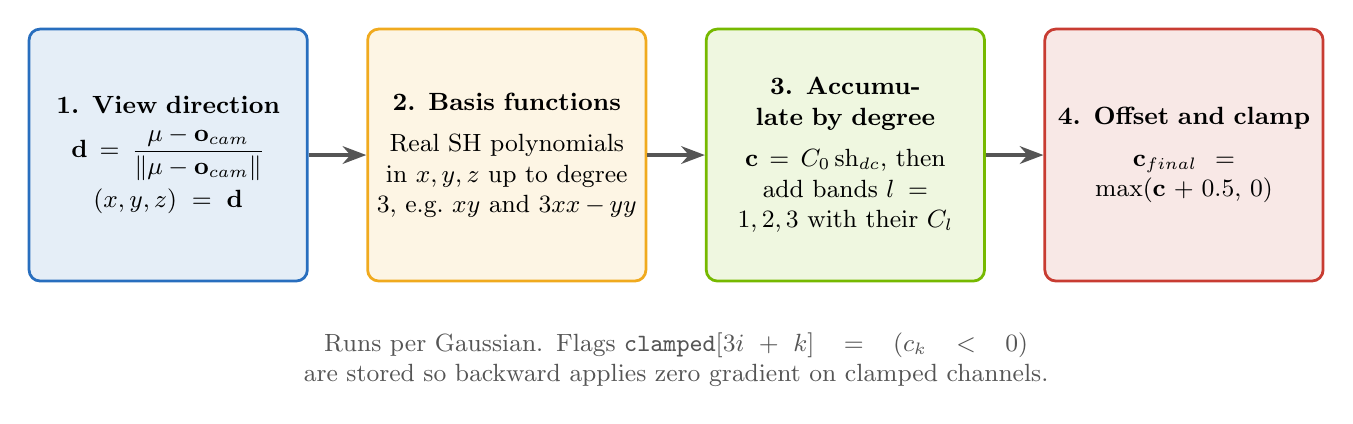
\begin{tikzpicture}[font=\sffamily]
  \tikzset{stp/.style={draw=#1,line width=1pt,rounded corners,fill=#1!12,minimum width=3.5cm,minimum height=3.2cm,align=center,font=\small,text width=3.3cm}}
  \node[stp=gsBlue] (s1) at (0,0) {\textbf{1. View direction}\\[4pt]$\mathbf d=\dfrac{\mu-\mathbf o_{cam}}{\lVert\mu-\mathbf o_{cam}\rVert}$\\[2pt]$(x,y,z)=\mathbf d$};
  \node[stp=pyYel] (s2) at (4.3,0) {\textbf{2. Basis functions}\\[4pt]Real SH polynomials in $x,y,z$ up to degree 3, e.g.\ $xy$ and $3xx-yy$};
  \node[stp=cudaG] (s3) at (8.6,0) {\textbf{3. Accumulate by degree}\\[4pt]$\mathbf c=C_0\,\mathrm{sh}_{dc}$, then add bands $l=1,2,3$ with their $C_l$};
  \node[stp=sadRed] (s4) at (12.9,0) {\textbf{4. Offset and clamp}\\[4pt]$\mathbf c_{final}=\max(\mathbf c+0.5,\,0)$};
  \foreach \a/\b in {s1/s2,s2/s3,s3/s4} {
    \draw[-{Stealth[length=3mm]},line width=1.2pt,secG] (\a) -- (\b);
  }
  \node[font=\small,secG,align=center,text width=13cm] at (6.45,-2.6) {Runs per Gaussian. Flags $\texttt{clamped}[3i+k]=(c_k<0)$ are stored so backward applies zero gradient on clamped channels.};
\end{tikzpicture}
\end{document}
